\chapter{Diskussion}\label{chap:d} 
Die Diskussion analysiert die Resultate der Methode, um daraus eine Antwort auf
die Fragestellung zu bilden. Zu diesem Zweck werden die einzelnen Unterfragen
dieser Arbeit behandelt. Darauf folgt ein Fazit und ein Ausblick zusammen mit
möglichen Anwendungsbereichen für die verschiedenen Versionen der künstlichen
Intelligenz.

\section{Diskussion der Fragestellung}\label{chap:d_frage} 
Die Fragestellung dieser Untersuchung lautet: Inwiefern kann eine künstliche
Intelligenz lernen, Strichbilder auf eine physische Weise nachzuzeichnen? Die
Unterfragen erfassen die verschiedenen Aspekte dieser Fragestellung und
erweitern diese sogar. Die Diskussion der Unterfragen macht somit die Antwort
auf die Fragestellung aus.

\subsection{Wie kann die Architektur einer KI aussehen, die das Nachzeichnen
erlernt?}\label{subsub:d_frage_unter_1} Das Deep Q-Learning Modell hinter der
nachzeichnenden KI erreicht hohe Werte in allen Kriterien und lässt sich, wie
die verschiedenen Variationen zeigen, auf der Grundlage von unterschiedlichen
Kriterien trainieren (siehe \doubleref{sub:r_tab_nachzeich}). Die Architektur
einer nachzeichnenden KI kann somit so aussehen, wie sie in dieser Arbeit
beschrieben ist (siehe \doubleref{chap:m_grund}).


\subsection{Wie lässt sich die Leistung der KI in ihrer Aufgabe
beurteilen?}\label{subsub:d_frage_unter_2} Die Leistung der KI lässt sich durch
fünf vordefinierte Kriterien beurteilen (siehe \doubleref{chap:m_eval}). Die
Werte der Kriterien sind quantifizierbar und automatisiert berechenbar, was sie
für die Anwendung in einer künstlichen Intelligenz geeignet macht. Allerdings
wären auch andere Kriterien denkbar, die das Nachzeichnen definieren. Dazu
gehören auch subjektive Definitionen, nach denen die KI das Nachzeichnen nicht
unbedingt erlernen kann. 

Unter den Kriterien ist die Erkennbarkeit ein Sonderfall, weil die Bestimmung
dieser auf eine klassifizierende KI angewiesen ist. Die klassifizierende KI
erreicht keine Genauigkeit von $100\%$ und schätzt wenige Zeichnungen aus der
Sicht der meisten Menschen falsch ein. Da die klassifizierende KI nicht perfekt
funktioniert, ist auch das Training der KI, in den Variationen wo diese
verwendet wird, nicht optimal. Aus diesem Grund sind auch die Resultate im
Kriterium der Erkennbarkeit minimal verfälscht. Die Verfälschung ist allerdings
sehr gering, da die klassifizierende KI je nach Typ eine Genauigkeit von bis zu
$98\%$ erreicht. Die klassifizierende KI für Buchstaben ist allerdings deutlich
schlechter mit einer Genauigkeit von $90\%$, was das Training und die Resultate
beeinflusst.

Die Kriterien der Geschwindigkeit, der zeichnenden Zeit und der Übermalung
werden verwendet, weil deren Kombination ein Mass für den `Schwung' in den
Bewegungen der KI gibt. `Schwung' heisst von einer subjektiveren Sichtweise, dass
die Zeichnungen schnell und möglichst in einem Ansatz fertiggestellt werden.



\subsection{Wie lässt sich die Leistung der KI in ihrer Aufgabe verbessern?}\label{subsub:d_frage_unter_3}
Die verschiedenen Variationen zeigen, dass ein spezifisches Training auf ein
Kriterium in den meisten Fällen die Leistung der nachzeichnenden KI in diesem
Kriterium erhöht. Einige Variationen sind dabei effektiver als andere:

%Todo: Change with results

Die \emph{Speed} Variation und dessen Kombination mit der \emph{No-Liftpen}
Variation erreichen die tiefsten Werte im Kriterium der Geschwindigkeit um $9$
Steps für das Nachzeichnen von Zahlen (siehe \doubleref{sub:r_tab_nachzeich}).
Diese Variationen können somit die Leistung der KI in ihrem ausgewählten
Kriterium verbessern.

Die \emph{Rec} Variation erreicht einen beinahe identischen Wert im Kriterium
der Erkennbarkeit wie die \emph{Base} Variation und einige andere. Diese
Variation konnte die Leistung somit nicht verbessern. Allerdings ist die
Erkennbarkeit mit $97\%$ für Zahlen der \emph{Base} Variation auch kaum
übertreffbar, vor allem weil die klassifizierende KI nur eine Genauigkeit von
$98\%$ erreicht.

Die \emph{No-Liftpen} Variation erreicht unter den Variationen die beste
Leistung im Kriterium der zeichnenden Zeit (siehe
\doubleref{sub:m_eval_zeichnend}) mit $98.1\%$ für das Nachzeichnen von Zahlen.
Die Variation erbringt somit den erwünschten Effekt.

Die \emph{Overdraw} erreicht unter den Variationen die tiefsten Werte im
Kriterium der Übermalung (siehe \doubleref{sub:m_eval_uebermalung}) mit $40$
übermalten Pixeln pro Zeichnung und kann somit ebenfalls die Leistung der KI
nach dem gewünschten Kriterium verbesseren.

Die \emph{Base} Variation erreicht die beste Leistung im Kriterium der
prozentualen Übereinstimmung, obwohl die meisten Variationen eine sehr ähnliche
Reward Function (siehe \doubleref{sub:m_var_base}) verwenden. Das deutet darauf
hin, dass in diesem Kriterium eine bessere Leistung erreicht wird, wenn die
Reward Function ausschliesslich für dieses Kriterium trainiert.

Die \emph{Physics} Variation verbessert die Leistung der nachzeichnenden KI
nicht. Für jedes Kriterium existieren andere Variationen, die deutlich bessere
Werte erreichen. Dieses Resultat deutet darauf hin, dass die KI mit den
Physiksimulationen nicht gut umgehen kann. Möglicherweise liegt das Scheitern
von diesem Ansatz daran, dass die Umgebung dadurch zu viele Faktoren hat, welche die
Bewegungen der KI beeinflussen.


\subsection{Wie ändert sich die Leistung der KI für Strichbilder, die im Training nicht enthalten sind?}\label{subsub:d_frage_unter_4} 
In allen Versionen bleibt die Leistung der KI zwischen den drei Datensets (siehe
\autoref{tab:models}) vergleichbar, wie die folgenden Tabellen (siehe
\autoref{tab:base-3-datasets} und \autoref{tab:speed-3-datasets}) zeigen.


%Todo: Waiting for Results

\begin{table}[!ht]
    \centering
    \caption{Vergleich der \emph{Base} Variation für die drei Datensets}\label{tab:speed-3-dataset}
    \begin{tabular}{|l|l|l|l|l|l|}
            \hline
            \hline ~ & Sim $[\%]$ & Rec $[\%]$ & Speed & Drawtime $[\%]$ & Overdrawn \\ \hline
            MNIST & 90.8 & 97.1 & 54.7 & 0.73 & 269 \\ \hline
            EMNIST & 89.6 & 85.0 & 60.5 & 81.9 & 315 \\ \hline
            QuickDraw & 81.8 & 93.7 & 56.5 & 73.9 & 227 \\ \hline
        \end{tabular}
\end{table}

\begin{table}[!ht]
    \centering
    \caption{Vergleich der \emph{Speed} Variation für die drei Datensets}\label{tab:speed-3-dataset}
    \begin{tabular}{|l|l|l|l|l|l|}
            \hline
            \hline ~ & Sim $[\%]$ & Rec $[\%]$ & Speed & Drawtime $[\%]$ & Overdrawn \\ \hline
            MNIST & 80.2 & 96.7 & 20.5 & 90.5 & 78 \\ \hline
            EMNIST & 78.0 & 77.0 & 32.6 & 92.2 & 130 \\ \hline
            QuickDraw & 74.5 & 85.7 & 29.5 & 89.3 & 93 \\ \hline
        \end{tabular}
\end{table}

Die Werte in den Tabellen stammen direkt aus den Resultaten und zeigen, dass es
im Vergleich der Leistung innerhalb einer Variation für die drei Datensets nur
geringe Unterschiede gibt. Vor allem für den Vergleich zwischen dem Quickdraw
Datenset und dem MNIST Datenset gilt diese Aussage. Für das EMNIST Letters
Datenset ist die Leistung der KI durchschnittlich in den meisten Kriterien etwas
tiefer.

Dieser Umstand könnte zum Grund haben, dass die Buchstaben aus dem EMNIST
Letters Datenset häufig deutlich dicker gemalt sind als die anderen Motive
(siehe \autoref{fig:emnist-mnist}). Ausserdem erreicht die klassifizierende KI
für Buchstaben eine niedrigere Genauigkeit als für Zahlen und QuickDraw-Motive
(siehe \autoref{tab:models}), wodurch die Leistung im Kriterium der
Erkennbarkeit stärker verfälscht wird als für die anderen Motive

%bild Noisy Pixel
\begin{figure}[!ht]
	\centering
	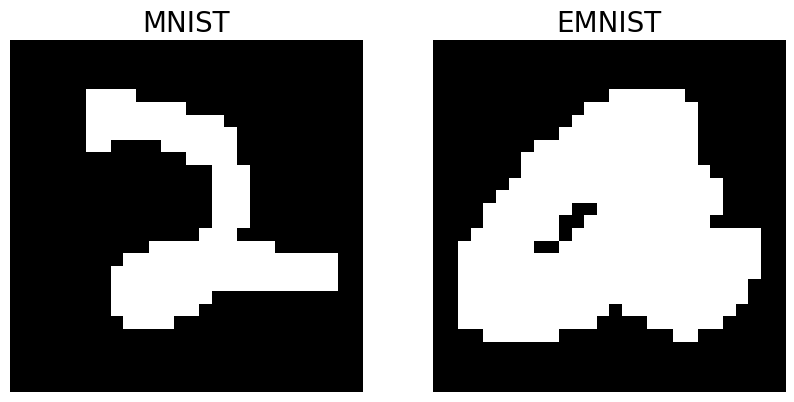
\includegraphics[width=\textwidth]{images/diskussion/emnist-mnist.png}
	\caption{Vergleich zwischen dem MNIST Datenset und dem EMNIST Datenset
	(eigene Abbildung)}\label{fig:emnist-mnist}
\end{figure}
  

\subsection{Wie und inwiefern lässt sich das Verhalten der KI mit menschlichem Zeichnen vergleichen?}\label{subsub:d_frage_unter_5}

Die nachzeichnende KI bewegt sich mit beschränkter Geschwindigkeit und kann nur
an dem Ort zeichnen, wo sie sich gerade befindet. Durch diese Einschränkungen in
der Freiheit der Bewegungen wären diese in die physische Welt übersetzbar.  Das
heisst, dass ein zeichnender Roboter prinzipiell mit der nachzeichnenden KI
bedienbar wäre.

Die \emph{Physics} Variation stellt einen Versuch dar, menschliches Zeichnen
weiter anzunähern. Dieser Versuch ist allerdings gescheitert, weil die KI
dadurch allgemein schlechter zeichnet als die anderen Variationen. die
\emph{Speed}, \emph{Rec} und \emph{No-Penlift} Variationen (siehe
\doubleref{chap:r}) nähern menschliches Zeichnen eher an, da diese Variationen
den `Schwung' der Bewegungen erhöhen. Schwung ist ein wichtiges Element für den
menschlichen Prozess des Zeichnens. Die \emph{Speed} Variation kommt insgesamt
dem menschlichen Zeichnen am nächsten, da diese in allen Kriterien gute Werte
erreicht und somit nicht nur mit `Schwung' zeichnet, sondern auch mit Präzision.


\subsection{Kann eine KI Strichbilder ohne Vorlage
zeichnen?}\label{subsub:d_frage_unter_6} Ja. Eine abgewandelte Form der
nachzeichnenden KI kann Strichbilder von einem ausgewählten Motiv zeichnen,
solange diese im Training mit dem gewähten Motiv trainiert. Beide Versionen der
generativen KI erreichen dabei eine Erkennbarkeit des gewünschten Motivs von
mehr als $90\%$. Die \emph{Random-Noise} errecht isgesamt marginal bessere
Werte.

Quantitativ gesehen erlernt die generative KI somit das Zeichnen von Motiven
ohne eine Vorlage. Eine subjektivere Einschätzung der generierteren Bilder
ergibt allerdings, dass die KI viele Motive nicht erkennbar nachzeichnet.
Besonderes das Motiv: F und das Motiv: Blume sind nicht immer erkennbar, selbst
wenn die klassifizierende KI diese so einschätzt. In dieser Fehleinschätzung
liegt das Hauptproblem der generativen KI. Wenn die klassifizierende KI ein Bild
falsch einschätzt, erhält die generative KI der Situation entsprechend falsche
Rewards. Die klassifizierende KI für Zahlen erreicht die höchste Genauigkeit
(siehe \ref{tab:models}) und aus diesem Grund zeichnet die KI Zahlen für
Menschen am besten erkennbar nach.

Der Test auf das Zeichnen von verschiedenen Zahlen spricht dafür, dass die
generative KI die meisten Motive nachzeichnen kann, solange diese mit einer
klassifizierenden KI mit einer hohen Zuverlässigkeit trainiert.

Da die KI ohne eine Vorlage eigene Zeichnungen produzieren kann, entwickelt sie
gewissermassen eine eigene Handschrift. Diese Tatsache stellt nicht nur einen
Fortschritt in der Nachahmung von menschlichem Verhalten durch Computer dar,
sondern gibt auch Einblicke darin, wie Menschen ihre Handschrift entwickeln. Es
stellt sich heraus, dass die KI dieser Arbeit nur lernen kann, eigene Bilder zu
zeichnen, wenn diese zuvor Beispiele vom gewünschten Motiv gesehen hat und das
Nachzeichnen von diesen Motiven erlernt hat. Das Lernen der künstlichen
Intelligenz gleicht somit dem Lernen von Kindern. Auch Kinder erlernen in ihren
ersten Schuljahren häufig das Schreiben von Zahlen und Buchstaben, indem sie
diese mit einem Stift nachfahren. Erst nachdem sie in dieser Aufgabe geübt sind,
beginnen die meisten Kinder, eigene Zeichen und Symbole zu Schreiben.


\section{Fazit und Ausblick}\label{chap:d_faz-aus} Die Resultate und deren
Interpretation in der Beantwortung der Unterfragen (siehe
\doubleref{chap:d_frage}) deuten darauf hin, dass verschiedene Variationen der
künstlichen Intelligenz das Nachzeichnen von beliebigen Strichbildern erlernt
haben. Diese Antwort unterliegt allerdings einigen Annahmen und Voraussetzungen,
die weiter diskutiert werden können. Beispielsweise ist das Format der
Strichbilder vorausgesetzt. Die KI kann in einem bestimmten Format beliebige
Bilder nachzeichnen, aber in einem anderen Format kann sie nicht zeichnen.
Spezifisch kann die KI kleine Bilder mit einer Auflösung von 28x28 Pixeln in
schwarzweiss und einer festen Strichbreite zeichnen. Diese Voraussetzungen
schränken die nachzeichnende KI ein, da viele Bilder nicht diesen
Voraussetzungen entsprechen. In der Aufhebung von diesen Einschränkungen liegt
Entwicklungspotenzial. Eine weitere Annahme liegt in der Definition des
Nachzeichnens. Die KI erlernt das nachzeichnen nach einer selbst bestimmten
Definition. Die Kriterien dieser Definition (siehe \doubleref{chap:m_eval}) sind
für den Trainingsprozess einer künstlichen Intelligenz sinnvoll gewählt, aber es
wären auch andere Kriterien denkbar.

Die Qualität der nachzeichnenden KI und der generativen KI hängt von der
Verlässlichkeit der klassifizierenden KI ab, die im Training verwendet wird. Da
diese nicht eine Genauigkeit von $100\%$ erreicht, ist das Training nicht
optimal. Ausserdem sind die Resultate im Kriterium der Erkennbarkeit durch die
Imperfektion der klassifizierenden KI leicht verfälscht.

Ausserdem sind die Hyperparameter von einigen Variationen der KI vermutlich
nicht optimal gewählt, da ein angemessener Optimierungsprozess zu viel
Rechenaufwand bedeuten würde. Die Leistung der KI liegt somit vermutlich leicht
unter ihrem vollen Potenzial.

Die generative KI kann ohne eine Vorlage selbstständig Zeichnungen produzieren
und entwickelt so in gewissem Sinne eine eigene Handschrift. Die nachzeichnende
KI ist ein entscheidender Vorläufer dieser KI, weil die generative KI zuerst das
Nachzeichnen erlernen muss, bevor sie selbstständig zeichnen kann. So erlernt
die KI das Zeichnen ohne Vorlage, indem sie zuerst aus verschiedenen Beispielen
lernt. Zu einem gewissen Grad adapiert die KI die Handschrift dieser Beispiele.
Da die KI allerdings mit tausenden Beispielen trainiert kann die Adaption und
Vermischung dieser auch als eine eigene Handschrift der KI angesehen werden.

Die generative KI kann hauptsächlich Symbole wie Zahlen und Buchstaben zeichnen.
Eine mögliche Erweiterung wäre, dass die KI das Schreiben von ganzen Wörtern
erlernt, weil ansonsten noch nicht von einer tatsächlichen Handschrift
gesprochen werden kann


\section{Anwendungsbereiche}\label{chap:d_anwendung} Für die nachzeichnende KI
und die generative KI sind nachfolgend einige Anwendungsbereiche beschrieben. Es
handelt sich dabei um Einsatzorte, bei denen diese künstlichen Intelligenzen
einen Nutzen bieten können.

Die Nachzeichnende KI könnte in der Robotik Anwendung finden. Die aktuelle
Version ist für diese Anwendung allerdings zu eingeschränkt, was die Art der
Bilder angeht, die sie zeichnen kann. Sollte eine weiterentwickelte Version
vielfältigere Bilder produzieren können, So würde ein Roboter mit der
nachzeichnenden KI von beliebigen Bildern Zeichnungen anlegen können.

Ein weiterer Anwendungsbereich der nachzeichnenden KI wäre die Vektorisierung.
Damit ist die Umwandlung von Rastergrafiken in Vektorgrafiken gemeint (siehe
\autoref{fig:vektorRaster}). Diese Konvertierung benötigt einen
Nachzeichenprozess. Die nachzeichnende KI kann für diese Aufgabe verwendet
werden. Um in der Praxis Anwendung zu finden, müsste die KI allerdings was den
Rechenaufwand angeht effizienter werden.

\begin{figure}[!ht]
	\centering
	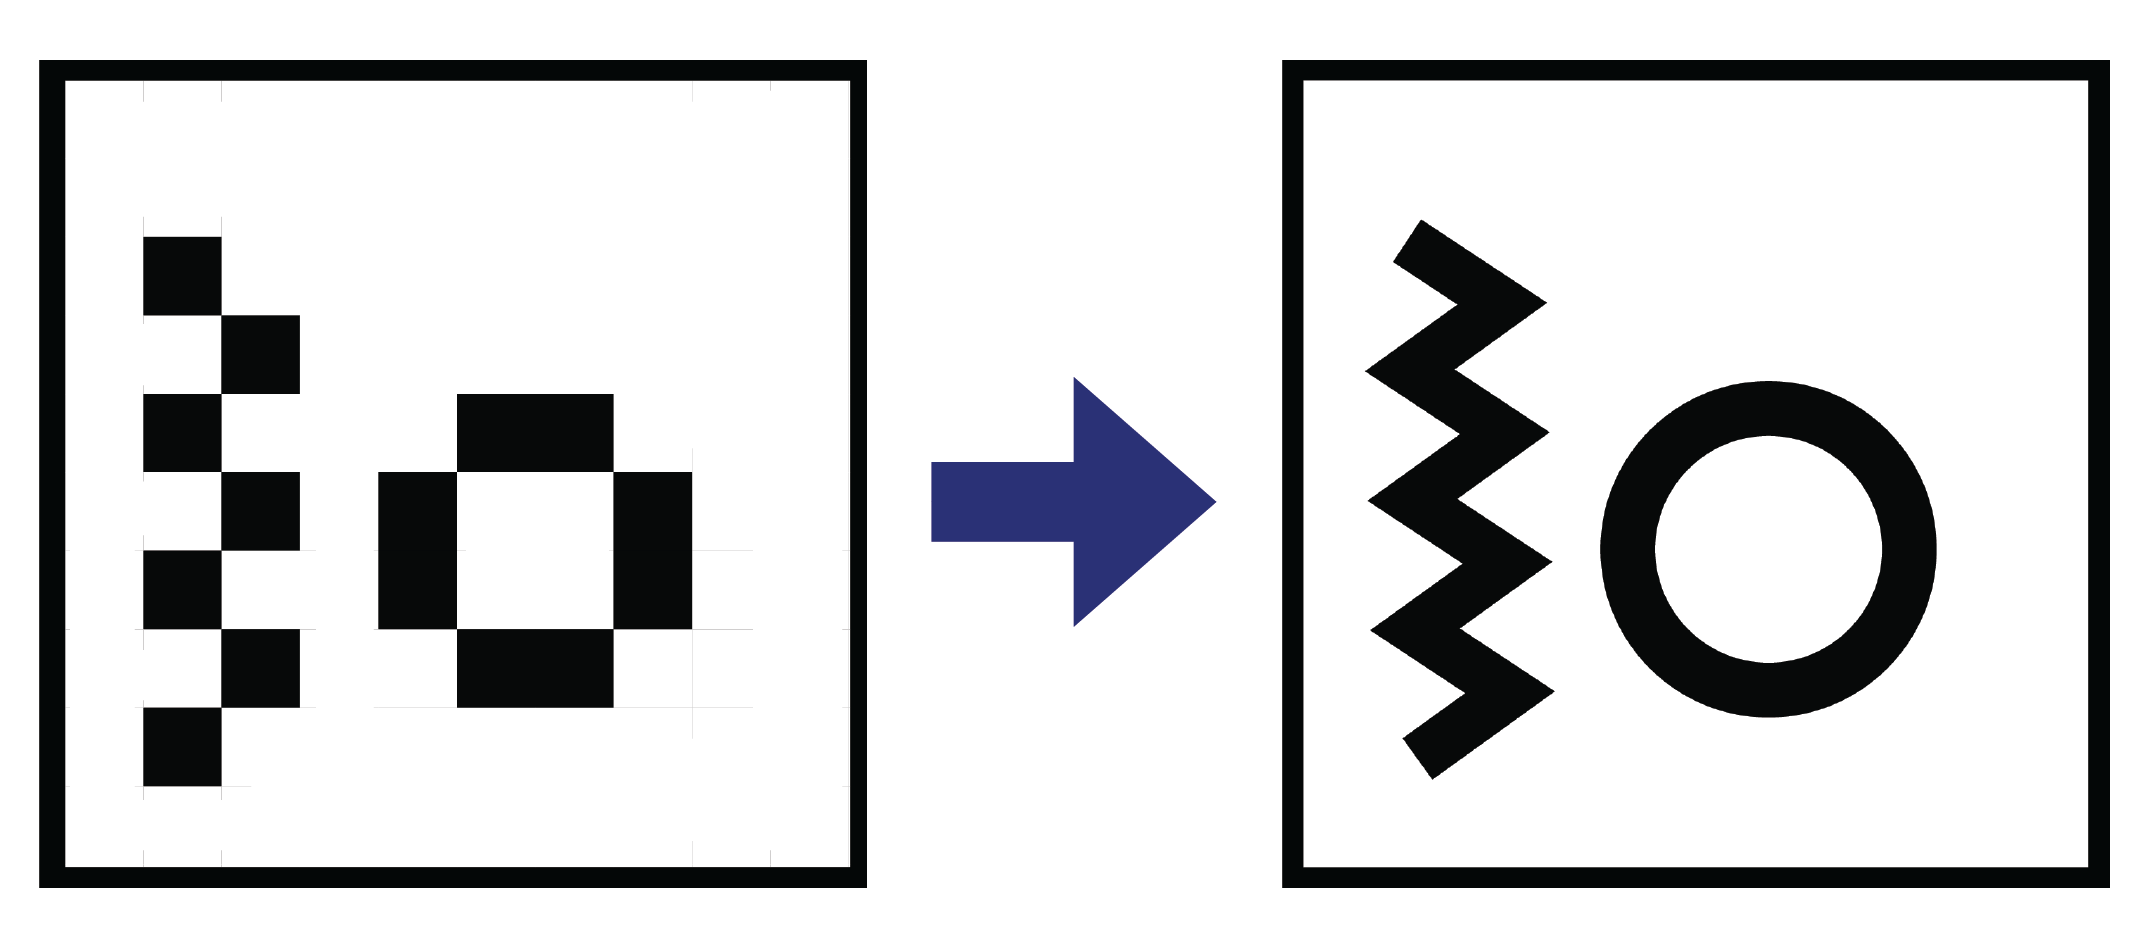
\includegraphics[width=\textwidth]{images/diskussion/Vector-Raster.png}
	\caption{Umwandlung von Rastergrafiken in Vektorgrafiken (eigene Abbildung)}\label{fig:vektorRaster}
\end{figure}

Eine Anwendung der Generativen KI wäre die Nachahmung von Handschriften. Wenn
der KI im Training zufällige Beispiele von einem Motiv gezeigt werden,
entwickelt die KI einen eigenen Weg um dieses Motiv zu zeichnen. Wenn der KI
allerdings Strichbilder von einer ausgewählten Person gegeben werden, würde die
KI die Handschrift dieser Person emulieren. Inwiefern die Zeichnungen der KI
tatsächlich der Handschrift einer Person entsprechen, ist allerdings nur
subjektiv bestimmbar.
